\chapter{ Challenges and Annotation Language Extension}
Main goal was to overcome the challenge of not being able
to detect implicit and explicit information flow bugs in UML state charts and C code. An annotation language
which can be used to annotate UML state charts and code by inserting information flow
restrictions during two software development phases (design
and coding). The insight was that the same annotation language can be used to add information flow constraints to UML state charts and code in order to detect information flow errors.
 
In this chapter the challenges and how the annotation language has extended are described.

\section{Challenges and Idea}

To develop the system eclipse xtext, eclipse xtend and static analysis engine named smtcodan(which is developed in Java to detect C and C++ vulneribilities) are used. For building the source code annotation editor eclipse xtext is used. Modeling the source as UML Statechart opensource platform YAKINDU SCT editor is used. Inside YAKINDU sct editor to genrate the .c(c file) and .h(header file) eclipse xtend is used mainly for genrating code files from statechart. Let's see in briefly what is xtext, xtend and how it works.

\begin{itemize}	
	\item Xtext : Xtext is a framework for development of programming languages and domain specific languages. According to the \cite{ref_17_xtext:grammar}, it covers all aspects of a complete language infrastructure, from parsers, over linker, compiler or interpreter to fully-blown top-notch Eclipse IDE integration. It comes with great defaults for all these aspects which at the same time can be easily tailored to individual user needs.
	
	Here is an example of xtext code:
		\begin{lstlisting} [caption={Xtext Code Example},label=lst:xtextCodeExample]
		grammar org.xtext.example.mydsl.MyDsl with 
		org.eclipse.xtext.common.Terminals
		
		generate myDsl "http://www.xtext.org/example/mydsl/MyDsl"
		
		Model:
		messages+=Message*;
		
		Message:
		'Hello' name=ID '!';
		
		\end{lstlisting}
		 
	This language allows to write down a list of messages. The following would be the proper input messages which are allowed to write:
		\begin{lstlisting}
			Hello User!
			Hello World!		
		\end{lstlisting}
		
	\textbf{How Xtext Works:}
	Xtext provides user with a set of domain-specific languages and modern APIs to describe the different aspects of user's programming language. Based on that information it gives user a full implementation of that language running on the JVM. The compiler components of user's language are independent of Eclipse or OSGi and can be used in any Java environment. They include such things as the parser, the type-safe abstract syntax tree (AST), the serializer and code formatter, the scoping framework and the linking, compiler checks and static analysis aka validation and last but not least a code generator or interpreter. These runtime components integrate with and are based on the Eclipse Modeling Framework (EMF), which effectively allows user to use Xtext together with other EMF frameworks like for instance the Graphical Modeling Project GMF.
	
	In addition to this nice runtime architecture, user will get a full blown Eclipse-IDE specifically tailored for user's language. It already provides great default functionality for all aspects and again comes with DSLs and APIs that allow to configure or change the most common things very easily. And if that's not flexible enough there is Guice to replace the default behavior with user's own implementations.
	
	\textbf{Domain-Specific Language:}
	A Domain-Specific Language (DSL) is a small programming language, which focuses on a particular domain. Such a domain can be more or less anything. The idea is that its concepts and notation is as close as possible to what you have in mind when you think about a solution in that domain. 
		
	The opposite of a DSL is a so called GPL, a General Purpose Language such as Java or any other common programming language. With a GPL you can solve every computer problem, but it might not always be the best way to solve it.
	
	Imagine a user want to remove the core from an apple. User could of course use a Swiss army knife to cut it out and this is reasonable if user have to do it just once or twice. But if user need to do that on a regular basis it might be more efficient to use an apple corer.
	
	There are a couple of well-known examples of DSLs. For instance SQL is actually a DSL which focuses on querying relational databases. Other DSLs are regular expressions or even languages provided by tools like MathLab. Also most XML languages are actually domain-specific languages. The whole purpose of XML is to allow for easy creation of new languages. Unfortunately, XML uses a fixed concrete syntax, which is very verbose and yet not adapted to be read by humans. Into the bargain, a generic syntax for everything is a compromise.
	
	Xtext is a sophisticated framework that helps to implement your very own DSL with appropriate IDE support. There is no such limitation as with XML, you are free to define your concrete syntax as you like. It may be as concise and suggestive as possible being a best match for your particular domain. The hard task of reading your model, working with it and writing it back to your syntax is greatly simplified by Xtext.
	
	\textbf{Users of Xtext:}
	Xtext is used in many different industries. It is used in the field of mobile devices, automotive development, embedded systems or Java enterprise software projects and game development. People use Xtext based languages to drive code generators that target Java, C, C++, C sharp, Objective C, Python, or Ruby code. Although the language infrastructure itself runs on the JVM, you can compile Xtext languages to any existing platform. Xtext based languages are developed for well known Open-Source projects such as Maven, Eclipse B3, the Eclipse Webtools platform or Google's Protocol Buffers and the framework is also widely used in research projects.
	
	\item Xtend : According to \cite{ref_20_xtend}, Xtend is a statically-typed programming language which translates to comprehensible Java source code. Syntactically and semantically Xtend has its roots in the Java programming language but improves on many aspects such as- Extension methods, Lambda Expressions, Active Annotations, Operator overloading, Powerful switch expressions, Multiple dispatch, Template expressions etc. Xtend has zero interoperability issues with Java: Everything you write interacts with Java exactly as expected. At the same time Xtend is much more concise, readable and expressive. Its small library is just a thin layer that provides useful utilities and extensions on top of the Java Development Kit (JDK). 
	
	\textbf{Java Interoperability:}
	Xtend, like Java, is a statically typed language. In fact it completely supports Java's type system, including the primitive types like int or boolean, arrays and all the Java classes, interfaces, enums and annotations that reside on the class path.
	
	Java generics are fully supported in xtend. User can define type parameters on methods and classes and pass type arguments to generic types just as user's are used to from Java. The type system and its conformance and casting rules are implemented as defined in the Java Language Specification.
	
	Resembling and supporting every aspect of Java's type system ensures that there is no impedance mismatch between Java and Xtend. This means that Xtend and Java are 100\% interoperable. There are no exceptional cases and you do not have to think in two worlds. You can invoke Xtend code from Java and vice versa without any surprises or hassles. As a bonus, if you know Java's type system and are familiar with Java's generic types, you already know the most complicated part of Xtend.
	
	The default behavior of the Xtend to Java compiler is to generate Java code with the same language version compatibility as specified for the Java compiler in the respective project. This can be changed in the global preferences or in the project properties on the Xtend  Compiler page (since 2.8). Depending on which Java language version is chosen, Xtend might generate different but equivalent code. For example, lambda expressions are translated to Java lambdas if the compiler is set to Java 8, while for lower Java versions anonymous classes are generated.
	
	\textbf{Type Inference:}
	One of the problems with Java is that you are forced to write type signatures over and over again. That is why so many people do not like static typing. But this is in fact not a problem of static typing but simply a problem with Java. Although Xtend is statically typed just like Java, you rarely have to write types down because they can be computed from the context.
	
	Consider the following Java variable declaration:
	\begin{lstlisting}
		final LinkedList<String> list = new LinkedList<String>();
	\end{lstlisting}
	The type name written for the constructor call must be repeated to declare the variable type. In Xtend the variable type can be inferred from the initialization expression:
	\begin{lstlisting}
		val list = new LinkedList<String>
	\end{lstlisting}
		
	Here is an example of xtend code:
	\begin{lstlisting} [caption={Xtend Code Example},label=lst:xtendCodeExample]
	package example	
	import java.util.List		
	class A {
	def greetToAll(List<String> names) {
		for(name: names) {
			println(name.helloMessage)
		}
	}
		
	def helloMessage(String name) {
		'Hello ' + name + '!'
		}
	}
	
	\end{lstlisting} 
	   
Xtend provides type inference, the type of name and the return types of the methods can be inferred from the context. Classes and methods are public by default, fields private. Semicolons are optional.
	
The example also shows the method helloMessage called as an extension method, like a feature of its first argument. Extension methods can also be provided by other classes or instances.
\end{itemize}


Previous annotation language grammer has been extended more
to detect implicit and explicit information flow bugs in UML
state charts and C code. The purpose of the same annotation language
can be used to add information flow constraints to UML state
charts and code in order to detect information flow errors.\\

The challenge was addressed by extending the annotation language containing textual annotations which can be used to annotate source code and UML state charts which are backward compatible. The single-line annotations have the same as previous consisting start tag "//@" and the multi-line annotations have the start tag "/*@" and the end tag "@*/" .\\

Some challenges throughout the approach are- converting textual
comments into annotations objects, introducing syntactically
correct annotations into files, how to use the same annotation
language in order to annotate UML state charts and source
code, dealing with scattered annotations and attaching annotations to the right function declaration or variable.\\

The eclipse xtext based grammar is used to parse the whole C/C++ language. The C/C++ source code file extensions (.h, .hh, .hhh, .hxx, .c, .cpp) and UML state chart annotation box (graphical boxes
which can be attached to different parts of a UML state chart diagram) can be annotated with policy language restrictions. The obtained CORE model (a one to one mapping from xtext grammar to the ECORE grammar representation) that can be reused for integrating the policy language into an UML state chart editor. Treating the annotation tags as EObjects created new possibilities for annotating
UML models. The policy language grammar has about 420 lines of code with code comments included. Source code generation is also supported by using
eclipse xtend, ANTLR and .mwe2 files. To parse other programming languages as well this annotation language parser can be used. The result is an extensible policy language and a highly reusable source code implementation as well as source code generator that can easily be used for annotating models and source files.

\section{Annotation Language Tags}
Table \ref{table:Security_language_annotation_tags} contains in this section: the annotation language
target types, the annotation tags which can be used in
combination with the tag @function, the tag
@parameter can be used to annotate the function parameter as authinticated/declassified/santized H/L and the tag @variable used to annotate the variable of C/C++ code with confiential H/L which are used to tag public and private variables. The tag @variable which can be used only inside single line annotations whereas @parameter is used only in multi line annotations. The tags were
defined and implemented iteratively based on the work flow
presented in figure \ref{figure:Language_Design_Process} and by using the eclipse xtext \cite{ref_17_xtext:grammar} language
definition grammar.\\

For detecting of authentication, declassification and sanitization errors new function tags included like authentication, declassification and sanitization function type. Also for parameter new tag type of parameter included such as authenticated, declassified and sanitized. Still H/L tags for parameter exists in the annotation tags for parameter to define that which type of parameter is this either \enquote{High} or \enquote{Low}. High means that this parameter is highly confidential or secured and low means that this parameter is not highly secured. The tag preStep used to annotate the previous function call name and tag postStep is used for next function call name. In Table \ref{table:Security_language_annotation_tags} the new tags for annotation language grammar has given with previous annotation tags. 

\begin{table}
	\centering
\begin{tabular}{|l|c|p{5cm}|}
	\hline
	Annotation Type   & Annotation Tag & Description  \\
	\hline

	@function         & sink  		   & uses information \\
	                  & source         & source provides information	\\
	                  & authentication & authentication authenticates information	\\
	                  & declassification& declassification declassifies information	\\
	                  & sanitization   & sanitization sanitizes information	\\
	                  & trust\_boundary& trust\_boundary is a trust-boundary\\ \hline

	@parameter        & authenticated H/L& authenticated-High/Low tags\\
					  & declassified H/L  & declassified-High/Low tags    \\
				      & sanitized H/L     & sanitized-High/Low tags    \\ \hline
	@variable         & confidential H/L & confidential-High/Low tags\\
					  & source H/L & source-High/Low tags   \\
	\hline
	
	@preStep         & preStep  & previous function call name\\ 	\hline
	@postStep        & postStep  & next function call name\\ 	\hline

	
\end{tabular}
\caption{Security language annotation tags}
\label{table:Security_language_annotation_tags}
\end{table}

\section{Annotation Language Implementation Process}

To implement the annotation language Eclipse Xtext \cite{ref_17_xtext:grammar} was used. Xtext is a sophisticated framework that helps to implement own DSL (Domain Specific Language) with appropriate IDE support. There is no such limitation as with XML, user's are free to define user's concrete syntax as user like. It may be as concise and suggestive as possible being a best match for user's particular domain. The hard task of reading user model, working with it and writing it back to user's syntax is greatly simplified by Xtext. Xtext relies heavily on Eclipse Modeling Framework (EMF) internally, but it can also be used as the serialization back-end of other EMF-based tools.  

Xtext provides a lot of generic implementations for language's infrastructure but also uses code generation to generate some of the components. Those generated components are for instance the parser, the serializer, the inferred Ecore model (if any) and a couple of convenient base classes for content assist etc. The generator also contributes to shared project resources such as the plugin.xml, MANIFEST.MF and the Guice modules. Xtext's generator uses a special DSL called MWE2 - the modeling workflow engine to configure the generator. MWE2 allows to compose object graphs declaratively in a very compact manner. The nice thing about it is that it just instantiates Java classes and the configuration is done through public setter and adder methods as one is used to from Java Beans encapsulation principles.

Xtext itself and every language infrastructure developed with Xtext is configured and wired-up using dependency injection. Xtext may be used in different environments which introduce different constraints. Especially important is the difference between OSGi managed containers and plain vanilla Java programs. To honor these differences Xtext uses the concept of ISetup (src)-implementations in normal mode and uses Eclipse's extension mechanism when it should be configured in an OSGi environment.

The Modeling Workflow Engine 2 (MWE2) is a rewritten backwards compatible implementation of the Modeling Workflow Engine (MWE). It is a declarative, externally configurable generator engine. Users can describe arbitrary object compositions by means of a simple, concise syntax that allows to declare object instances, attribute values and references. One use case - that's where the name had its origins - is the definition of workflows. Such a workflow consists usually of a number of components that interact with each other. There are components to read EMF resources, to perform operations (transformations) on them and to write them back or to generate any number of other artifacts out of the information. Workflows are typically executed in a single JVM. However there are no constraints the prevent implementors to provide components that spawn multiple threads or new processes.

Xtext ships with a default set of predefined, reasonable and often required terminal rules. The grammar for these common terminal rules is defined as follows:
	\begin{lstlisting}
		grammar org.eclipse.xtext.common.Terminals 
		hidden(WS, ML_COMMENT, SL_COMMENT)
		import "http://www.eclipse.org/emf/2002/Ecore" as ecore
		terminal ID : 
		'^'?('a'..'z'|'A'..'Z'|'_')('a'..'z'|'A'..'Z'|'_'|'0'..'9')*;
		terminal INT returns ecore::EInt: 
		('0'..'9')+;
		terminal STRING  : 
		'"' ( '\\'('b'|'t'|'n'|'f'|'r'|'u'|'"'|"'"|'\\') | !('\\'|'"') )* '"' |
		"'" ( '\\'('b'|'t'|'n'|'f'|'r'|'u'|'"'|"'"|'\\') | !('\\'|"'") )* "'"; 
		terminal ML_COMMENT  : 
		'/*' -> '*/';
		terminal SL_COMMENT : 
		'//' !('\n'|'\r')* ('\r'? '\n')?;
		terminal WS  : 
		(' '|'\t'|'\r'|'\n')+;
		terminal ANY_OTHER: 
		.;
	\end{lstlisting}

In order to implement the annotation language grammer in this research it was required to extend the terminal rule ML\_COMMENT and SL\_COMMENT. After extending these two rules it looks like this:

\begin{lstlisting}
	/**
	* @SL_COMMENT :all strings which follow // | || | } will be a single line comment
	*/ 
	terminal SL_COMMENT 	: '//'!('@')  !('\n'|'\r')* ('\n'|'\r')*
	// '}' can be used optional to disable the method bodyes together with multiline line {} comment 
	//     | '}'         !('\n'|'\r')* ('\n'|'\r')*               
	;
	
	/**
	* @ML_COMMENT :@/* multiline comment excluding @ from inside
	*            :{} multi line comment 
	*/ 
	terminal ML_COMMENT	: '/*' !('@') -> !('@')'*/'   !('\n'|'\r')* ('\n'|'\r')*   
	// '{' -> '}' can be used optional to disable the method bodies together with single line { comment 
		//      | '{' -> '}'                   ('\n'|'\r')?
		;   
\end{lstlisting}

The process depicted in figure \ref{figure:Language_Design_Process} was used in order to
implement annotation language. Figure 3.1 depicts the
annotation language implementation process. The process is
comprised of the following steps: At first, the .xtext file
containing the language grammar was extended following the requirements. Next the grammar file is compiled and software artifacts are generated. After editing the .mwe2 file then compile it. The result of compiling is: a parser, a lexer and class bindings between these two (lexer and parser) and the grammar ECore model. The generated parser, lexer and the bindings were reused inside static analysis engine and in the UI source file editor. After opening and editing a source file with the editor,the file can be parsed and the annotations can be automatically loaded and used inside checkers.
\begin{figure}[htbp]
	\centering
	\makebox[\textwidth]{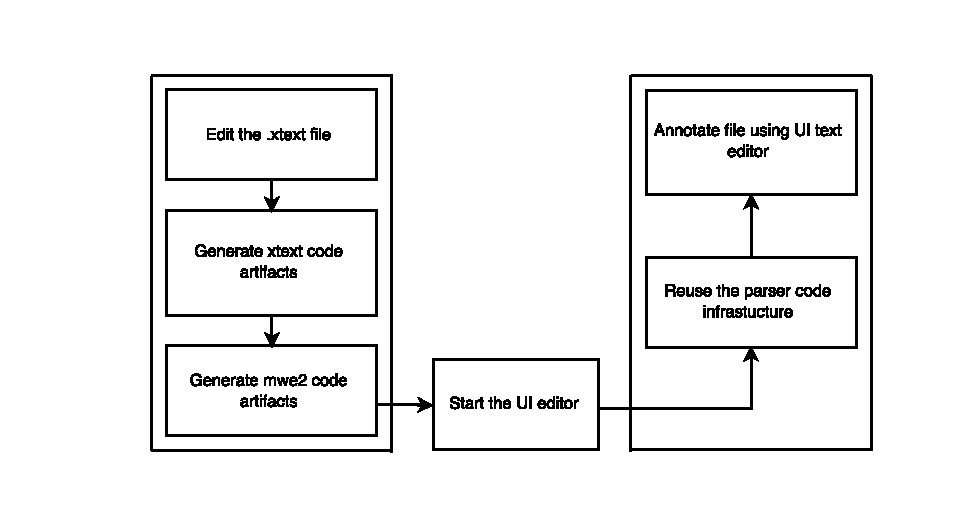
\includegraphics[width=\textwidth,scale=.50]{styles/Language_Design_Process.pdf}}
	\caption{Annotation language design process}
	\label{figure:Language_Design_Process}
\end{figure}